\label{partie_architecture}
L'application est conçue selon le \textit{modèle en couche}, bien qu'elles ne soient pas strictes.
Elle n'utilise \underline{pas} le pattern MVC
\footnote{\label{MVC_pas_utile}Pattern pour les applications disposant de vues.
  Les dépendances ne sont pas les mêmes que pour le modèle en couche.}.
L'architecture globale est expliquée dans cette section, les paquetages sont un peu plus détaillées ensuite si nécessaire.

\begin{figure}[!h]
  \centering
  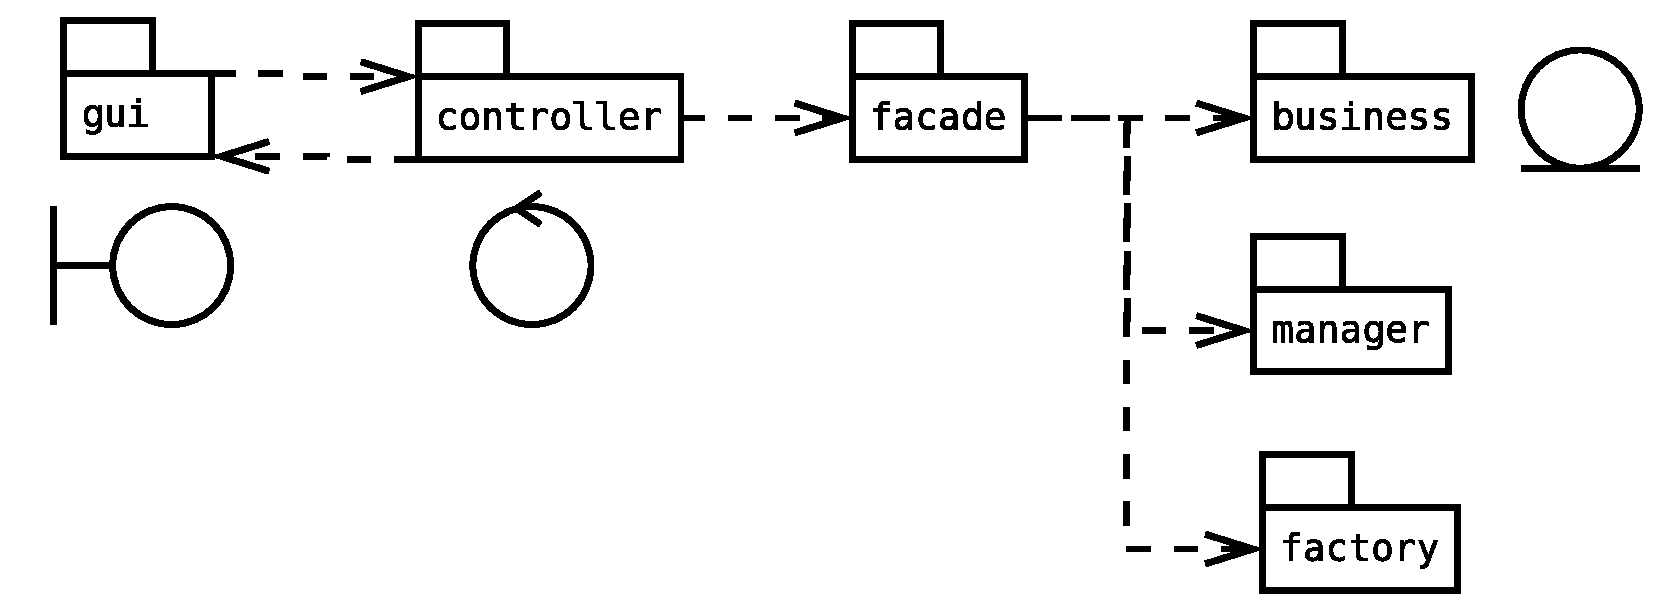
\includegraphics[width=14cm]{images/paquetage.eps}
  \caption{Diagramme de paquetage de l'application.}
  \label{diagramme_de_paquetage_idb}
\end{figure}

\subsection{Couche présentation}
La couche \textit{présentation} contient les IHM de l'application.
Le code des classes ne contient que ce qui est nécéssaire pour l'agencement et le paramétrage des composants sur la vue.

Sur la figure \ref{diagramme_de_paquetage_idb}, la couche présentation se trouve dans le paquetage \textit{gui} (Graphic User Interface, IHM en français).

\subsection{Couche contrôle}
La couche \textit{contrôle} contient l'\textit{intelligence} des IHM, c'est à dire ce qu'il doit se passer \textbf{hors} de la vue (dans les bases de données, la RAM etc.) après un clic sur tel ou tel bouton, case à cocher ou tout autre composant.

Cette couche décharge le code des IHM et fait office d'\textit{indirection} entre les vues et le reste de l'application : les IHM ne connaissent que leurs contrôleurs respectifs.

Sur la figure \ref{diagramme_de_paquetage_idb}, la couche contrôle se trouve dans le paquetage \textit{controller}.
Comme le montre le diagramme, les dépendances entre les paquetages \textit{gui} et \textit{controller} ne sont pas unilatérales.
C'est trompeur : en réalité, les contrôleurs connaissent leurs IHM uniquement pour éviter de les afficher en double.
Il était possible de faire des IHM des \textit{singletons}, cependant cela n'aurait pas réglé le défaut du \textit{fort couplage}.

Les IHM ne sont donc pas des singletons et les contrôleurs y sont associés (au sens UML du terme).

\subsection{Couche entité}
La couche \textit{entité} ou \textit{métier} contient la valeur ajouté de l'application, c'est à dire toutes les classes dont le code génère le service de l'application.

Dans ce projet tuteuré, les classes métiers sont une pseudo-couche \gls{orm}
\footnote{\label{faux_orm}Les ORM convertissent les données en objets, dans cette application se sont les \textit{conteneurs} des données qui sont convertis en objets.}
qui représentent les tables et les contraintes du SGBD connecté à l'application.
Elles limitent les accès réseaux au SGBD, ce qui augmente les performances de l'application, et participent à la génération de code SQL à partir des saisies faites dans les IHM.

Sur la figure \ref{diagramme_de_paquetage_idb}, la couche métier se trouve dans le paquetage \textit{business}.

\subsection{Couche facade}
La couche \textit{facade} reprend le \textit{design pattern} façade.
Son utilité est de limiter les dépendances entre les contrôleurs et les autres paquetages de l'application.
Elles n'apportent rien d'autres à l'application.

Sur la figure \ref{diagramme_de_paquetage_idb}, la couche facade se trouve dans le paquetage \textit{facade}.

Les figures \ref{trois_premières_couches} et \ref{facades_et_managers} montrent les intéractions entre les façades et les paquetages dont elles cassent les dépendances avec les contrôleurs. Les couleurs sont indépendantes d'une figure à l'autre, elles distinguent :
\begin{itemize}
\item les couches présentation, contrôle et façade sur la figure \ref{trois_premières_couches},
\item les associations entre les façaces et les autres classes sur la figure \ref{facades_et_managers}.
\end{itemize}

\begin{figure}[!h]
\centering
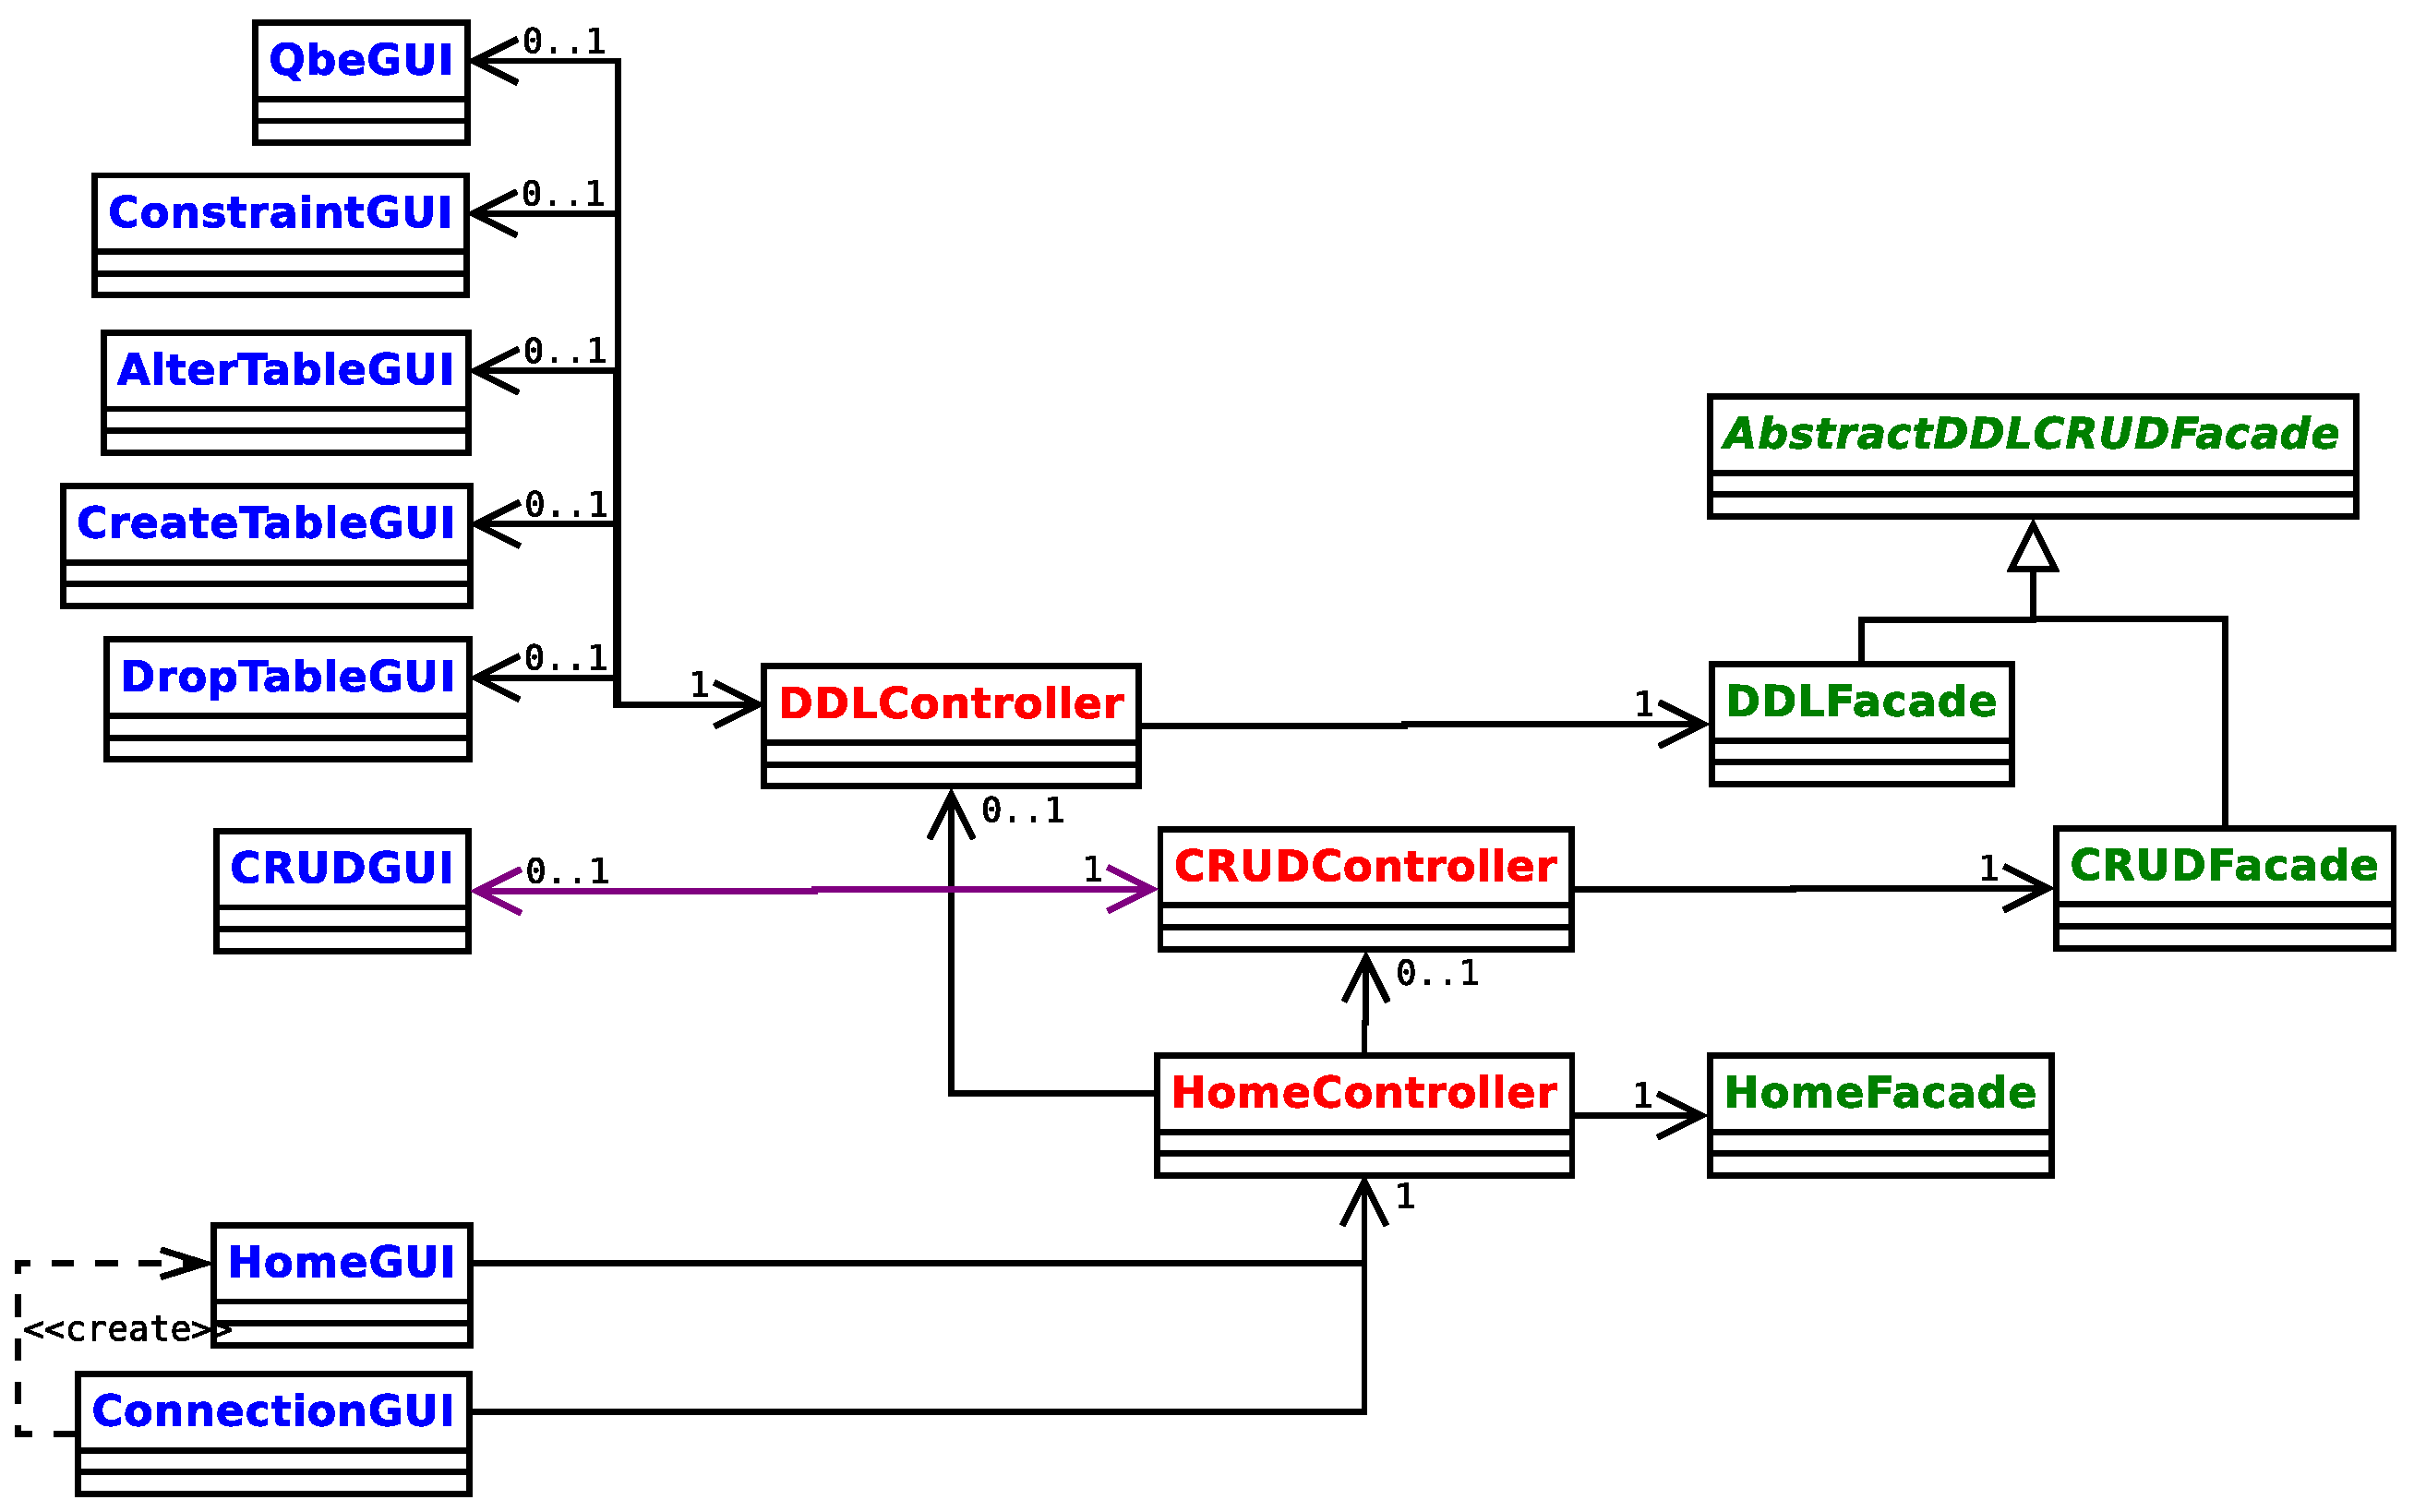
\includegraphics[width=14cm]{images/facades_crud_ddl.eps}
\caption{Couches présentation, contrôleur et façade.}
\label{trois_premières_couches}
\end{figure}

\begin{figure}[!h]
\centering
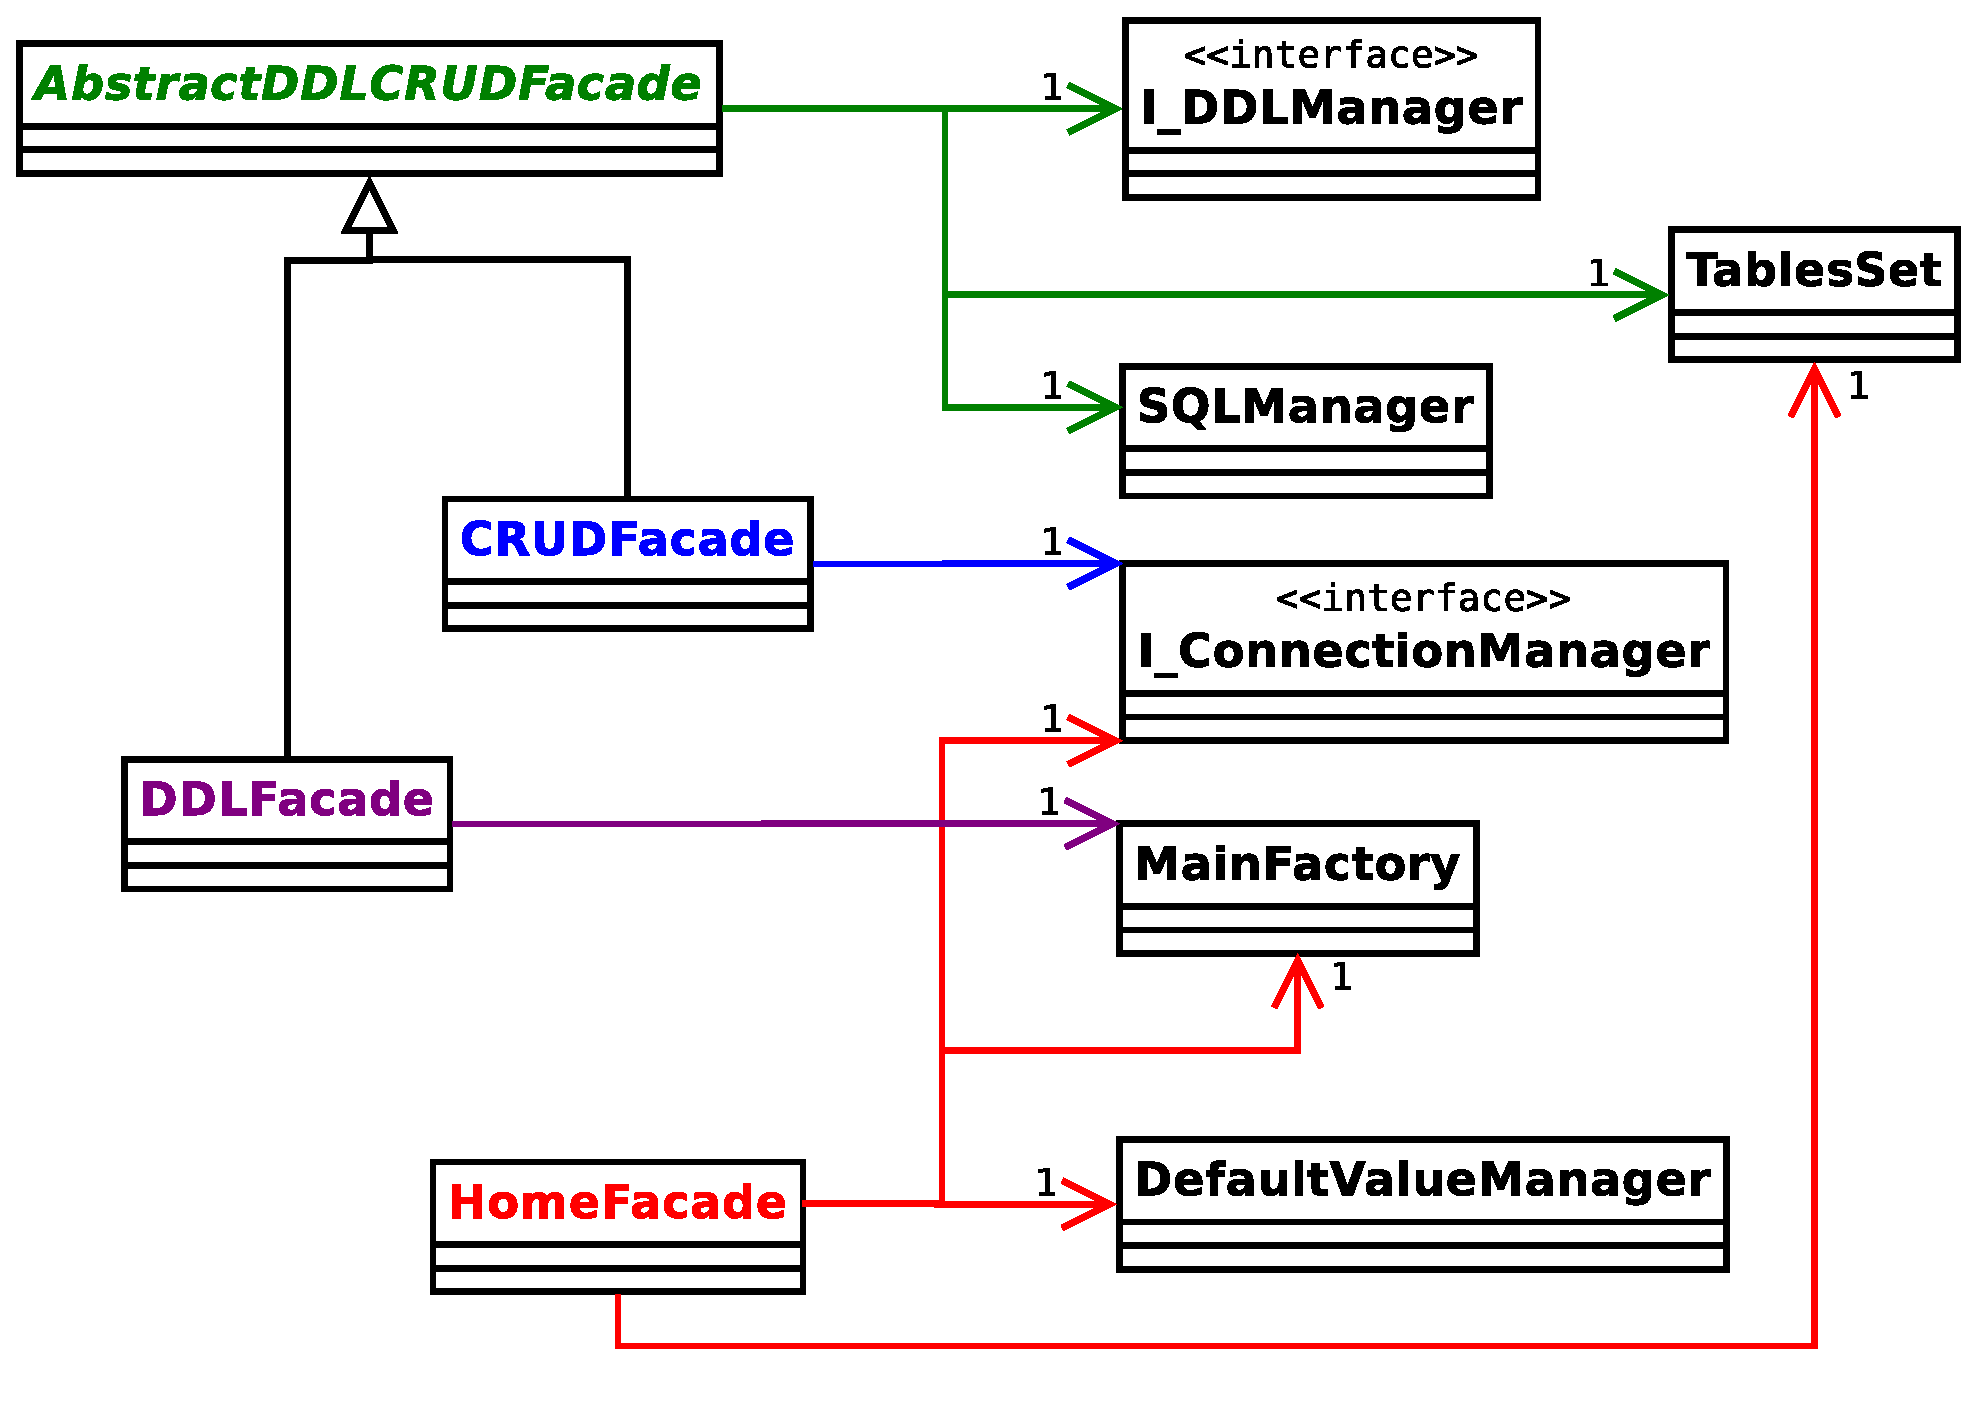
\includegraphics[width=14cm]{images/facades_managers.eps}
\caption{Intéractions entre les façades et les autres paquetages.}
\label{facades_et_managers}
\end{figure}

\subsection{Couche DAO}
La couche \gls{dao} permet d'enregistrer et récupérer des informations depuis le SGBD.
En temps normal, les DAO permettent d'enregistrer des données.
Dans cette application, ils permettent d'enregistrer les données, leurs conteneurs (tables) et les \glspl{constraint}.
Ils ont également un rôle de générateur de code SQL, généralement "simple" et qui diffère selon le SGBD connecté, contrairement aux classes métiers qui fournissent du SQL qui fonctionne sur tous les SGBD.

Sur la figure \ref{diagramme_de_paquetage_idb}, la couche DAO se trouve dans le paquetage \textit{manager}.
Les DAO sont utilisés \textit{à peu près} en suivant le design pattern \textit{data mapper}
\footnote{\label{faux_data_mapper}Ce pattern stipule que ce soient les classes qui \underline{utilisent} les \gls{orm} qui les enregistrent dans un système de stockage.}
, dans le sens où ce sont les contrôleurs de l'application qui les utilisent (par le biais des façades) pour enregistrer les tables et ce qu'elles contiennent.


